\documentclass{beamer}

\usepackage{ucs}
\usepackage[utf8x]{inputenc}
\usepackage[T1]{fontenc}
\usepackage[english]{babel}
\usepackage{epstopdf}
\usepackage{algpseudocode}
%\usepackage{algorithmicx}
\usepackage{algorithm}

\usepackage{subfig}
\usepackage{algpseudocode}
\usepackage{algorithmicx}
\usepackage{algorithm}
\usepackage{relsize}%	relative font sizes
\usepackage{multicol}
\usepackage{multirow}
\usepackage{todonotes}
\usepackage{xspace}
\newcommand{\computeflux}{\texttt{compute\_flux}\xspace}
\newcommand{\update}{\texttt{update}\xspace}
\newcommand{\polu}{\texttt{polu}\xspace}
\newcommand{\dirichlet}{\textit{Dirichlet}\xspace}

\graphicspath{{../images/}}


%	presentation info
\title[CUDA Profiling]{A Comparative and Critical Analysis on CUDA Profiling}

\author[M. Palhas, P. Costa]{Miguel~Palhas \and Pedro~Costa}

\institute[pg19808,pg19828]{
	Department of Informatics\\
	University of Minho
}

\date{Braga, July 2012}


%	beamer options
\usetheme{CambridgeUS}

\begin{document}%	begin presentation

\frame[plain]{\titlepage}

%\frame{\frametitle{Index}\tableofcontents}

\frame{\tableofcontents}

\section{Profiling: CPU vs GPU}

\frame{
	\frametitle{GPU Profiling}

	\begin{block}{What can be done}
		Gather GPU specific data
			\begin{itemize}
				\item Hardware counters
				\item Global GPU activity
			\end{itemize}

		Analyse and prove code improvements
	\end{block}

	\begin{block}{What can't be done}
		Compare CPU vs GPU implementations (except for global speedups)
	\end{block}
}

\frame{
	\frametitle{GPU Profiling}

	\begin{block}{Limitations}
		\begin{itemize}\itemsep=10pt
			\item Several Streaming Multiprocessors, but not all area measured
				\begin{itemize}
					\item Before Compute Capability 2.0, only 1 SM was measured
					\item Later versions measure more than one (but still not all!)
				\end{itemize}
			\item Harder to profile heterogeneous kernels

			\item Counters have different domains. Results may overlap

			\item Multi-context CUDA apps still lack support
		\end{itemize}
	\end{block}
}
\section{Command Line Profiler}

\frame{
	\frametitle{Command Line Profiler}

	
	Provides basic profiling, based on hardware counters

	\begin{block}{Advantages}
		\begin{itemize}
			\item Almost no setup required

			\item Fast results to use as starting point

			\item Good starting point for deeper analysis
		\end{itemize}
	\end{block}

	\begin{block}{Disadvantages}
		\begin{itemize}
			\item Useful only for small/fast results

			\item Output format too simple for more complex requirements
		\end{itemize}
	\end{block}
}
\section{Visual Profiler}

{
	\usebackgroundtemplate{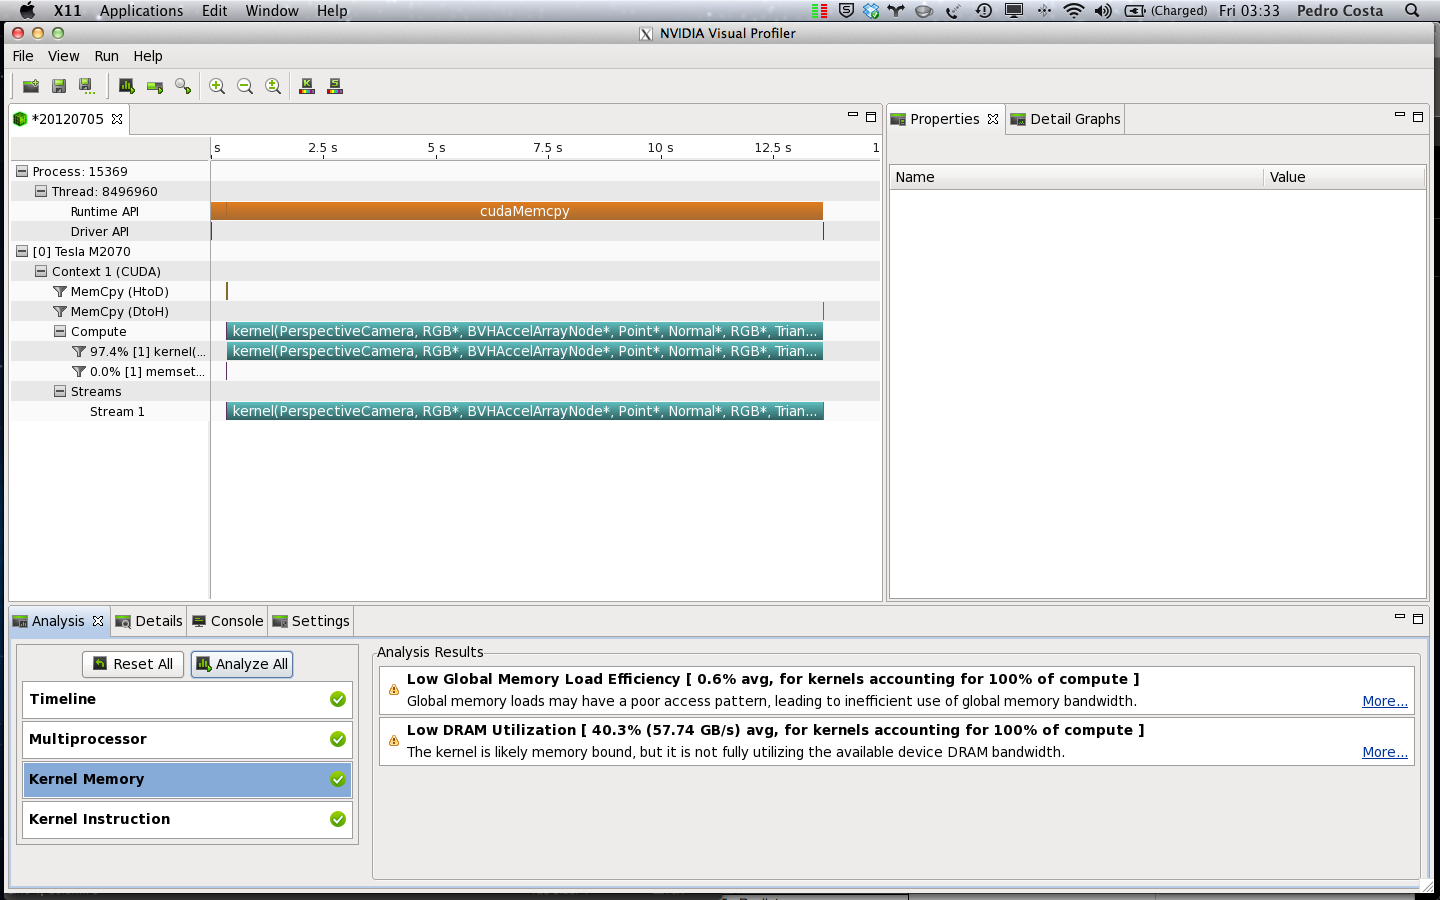
\includegraphics[width=\paperwidth,height=\paperheight]{../images/visprof.png}}
	\frame[plain]{}
}

\begin{frame}
	\frametitle{Visual Profiler}
	\begin{itemize}
		\item Similar to the Command Line Profiler;
		\begin{itemize}
			\item More organized;
			\begin{itemize}
				\item Functions Timeline;
				\item Function Properties;
				\item Detailed Graphs;
			\end{itemize}
			\item Same profiler counters;
		\end{itemize}
		\item Automatic operations;
		\item Automatic analysis;
		\item Executes several times for completeness;
		\item Not as detailed or extensive as CUPTI.
	\end{itemize}
\end{frame}
\section{CUPTI}

\frame{
	\frametitle{CUPTI}

	\begin{block}{What is it?}
		\begin{itemize}
			\item Provides a set of APIs for low-level driver calls

			4 different APIs are available:
			\begin{itemize}
				\item \textbf{Activity}
				\item \textbf{Callbacks}
				\item \textbf{Events}
				\item \textbf{Metrics}
			\end{itemize}
		\end{itemize}
	\end{block}


	\begin{block}{What is it for?}
		For applications requiring more extensive and customized profiling.
		\\
		Not for the faint of heart
	\end{block}
}

\frame{
	\frametitle{CUPTI}

	\begin{itemize}\itemsep=15pt
		\item Exposes CUDA driver to the programmer

		\item Allows low level manipulation and profiling

		\item Callbacks allow for overhead-free measurements

		\item \larger\textbf{Properly documented!}
	\end{itemize}
}
\section{PAPI CUDA}

\begin{frame}
	\frametitle{PAPI CUDA}
	\begin{itemize}
		\item Uses CUPTI;
		\begin{itemize}
			\item Supposed to be a wrapper;
		\end{itemize}
		\vfill
		\item [+] Approach to GPU counters is similar to CPU;
		\vfill
		\item [-] Requires the same ``garbage'' code;
		\vfill
		\item Works best when used with CUPTI Callbacks;
		\begin{itemize}
			\item It should replace them;
			\item Tests performed only obtained the measurements for the global kernel;
			\begin{itemize}
				\item Subkernels were ignored;
				\item Highly verbose preparation does not allow to discard programmer error;
			\end{itemize}
		\end{itemize}
		\vfill
		\item \textbf{\larger No documentation at all available!}
	\end{itemize}
\end{frame}

\section{Conclusions}

\frame{
	\frametitle{Conclusions - NVidia profilers}

	\begin{itemize}\itemsep=15pt
		\item 3 official profiling methodologies
			\begin{itemize}
				\item \textbf{Command Line}: Fast to use
				\item \textbf{Visual Profiler}: More user friendly
				\item \textbf{CUPTI}: Full driver access
			\end{itemize}

		\item Each one can have different purposes/applications

		\item Given their purpose, they get the job done

		\item Limitations come mostly from Hardware and/or Driver
	\end{itemize}
}

\frame{
	\frametitle{Conclusions - PAPI CUDA}

	\begin{itemize}\itemsep=15pt
		\item Attempt to wrap CUPTI in a known API

		\item Small subset of its features (Callbacks seems crutial!)

		\item Will probably fail at profiling asynchronous or multi threaded applications

		\item Still requires CUPTI's help for more complex tasks
		\begin{itemize}
			\item[-] \textit{So why not just use CUPTI instead?}
		\end{itemize}

		\item \textbf{No documentation at all}
	\end{itemize}

}



\begin{frame}[plain]
	\titlepage
	\begin{center}
		\Huge\bfseries - ? -
	\end{center}
\end{frame}

\end{document}%	end presentation